\section{Analysis}
\label{sec:analysis}

\subsection{PEFT Conditioning Produces Target-Specific Subsets}

The reuse experiment showed that a single fixed subset cannot serve a registry; this section shows the converse mechanism---that PCU-Select's one reusable scorer produces a \emph{different} subset for each configuration without recomputing per-target gradients. Appendix Figure~\ref{fig:config-sensitivity} tests whether the PEFT code changes behavior inside the same LoRA family. PCU-Select achieves 21.25 average performance across the configuration scan, compared with 20.70 for LESS, 20.27 for RDS+, and 18.82 for random. The mismatch matrix shows that using the subset selected for the correct target configuration is better than reusing a subset selected for a different configuration by 1.45 points on average. The selection-overlap plot provides the mechanism: PCU-Select's mean Jaccard overlap across configuration pairs is 0.427, while RDS+ remains 0.981 because it is PEFT-agnostic; the overlap broken down by structural axis (rank, placement, module set, family) is in Appendix Table~\ref{tab:overlap}. The Spearman correlation between the ordinal configuration distance and PCU-Select's selection difference is $\rho=0.71$ (95\% CI $[0.52, 0.83]$), confirming that the selection responds to structural distance rather than to noise.

\begin{figure}[H]
\centering
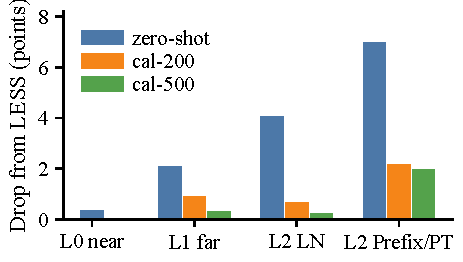
\includegraphics[width=.78\columnwidth]{Figures/fig_ood_calibration.pdf}
\caption{OOD transfer and calibration. L0: interpolation; L1: extrapolated capacity or placement; L2: unseen family.}
\label{fig:ood-calibration}
\end{figure}

\subsection{Ablations Identify the Useful Components}

\begin{table}[!b]
\centering
\small
\setlength{\tabcolsep}{4pt}
\begin{tabular}{lrrr}
\toprule
Variant & Metric & Drop & NDCG \\
\midrule
Full PCU-Select & 19.72$\pm$0.22 & 0.00 & 0.702 \\
No PEFT code & 18.35$\pm$0.41 & 1.37 & 0.526 \\
Family one-hot only & 19.04$\pm$0.29 & 0.68 & 0.602 \\
No task sketch & 18.90$\pm$0.31 & 0.82 & 0.597 \\
No activation signature & 19.24$\pm$0.25 & 0.48 & 0.629 \\
Gradient-proxy labels only & 18.87$\pm$0.34 & 0.85 & 0.563 \\
Short-update labels only & 19.36$\pm$0.27 & 0.36 & 0.639 \\
No uncertainty penalty & 19.44$\pm$0.24 & 0.28 & 0.690 \\
Global top-$k$ & 18.64$\pm$0.38 & 1.08 & 0.684 \\
Uniform clusters & 19.21$\pm$0.28 & 0.51 & 0.709 \\
\bottomrule
\end{tabular}
\caption{Ablations on GSM8K and HumanEval with two representative PEFTs at a 10\% budget (task-native metric averaged over the two tasks, mean$\pm$SD over three seeds). Drop is relative to the full adaptive selector; we measure NDCG against held-out short-update labels.}
\label{tab:ablations}
\end{table}


Table~\ref{tab:ablations} shows that the largest drop comes from removing the PEFT code: performance falls by 1.37 points and, most tellingly, ranking NDCG against held-out utility labels collapses from 0.702 to 0.526---a scale-free signal that the PEFT condition is what lets the scorer order examples correctly. Replacing the structured PEFT code with a family one-hot vector loses 0.68 points, which confirms that rank, placement, capacity, and recipe matter beyond the family name. Removing the task sketch loses 0.82 points, showing that PCU-Select also learns task relativity. Multi-fidelity supervision also matters: low-fidelity-only training loses 0.85 points, while high-fidelity-only training loses 0.36 points because it lacks broad coverage. The adaptive cluster selector beats global top-$k$ by 1.08 points and uniform cluster quotas by 0.51 points. The uniform-cluster variant is instructive: its ranking NDCG ($0.709$) slightly exceeds the full selector's ($0.702$) yet its downstream metric is lower, because equal per-cluster quotas over-sample low-value clusters---ranking quality and subset quality optimize different objectives. The appendix per-task analysis studies the two cells where PCU-Select trails LESS: TyDiQA and MLP-only LoRA.

\subsection{Transfer Protocol for Unseen PEFTs}

The offline scorer serves the seen registry directly, but a deployed system also meets targets outside it, so we turn the OOD analysis into a deployment protocol keyed on a cheap test. A Mahalanobis distance from the seen configuration distribution over $z_p$ assigns each new target to one of three tiers before any labels are drawn: L0 is interpolation (rank/capacity between seen values), L1 is extrapolation (capacity or placement beyond the seen range), and L2 is an unseen PEFT family (Prefix, P-Tuning, BitFit). Because only five seen configurations define the training distribution, the $z_p$ covariance is shrinkage-regularized and the Mahalanobis distance is used coarsely, as a tier assignment rather than a precise density estimate. Zero-shot PCU-Select is within 0.34 points of LESS at L0, trails by 2.08 at L1 (500 calibration labels recover 1.78), and trails by 5.76 at L2 (500 labels recover 5.53); calibration costs 2.1 GPU-hours per target (500 labels through the same $1.89$\,s-per-triple high-fidelity routine used offline), still small relative to a full LESS recomputation. The protocol follows directly (Table~\ref{tab:protocol}): interpolated targets transfer zero-shot, extrapolated targets take a few hundred calibration labels, and unseen families must be calibrated before the scorer is trusted. Calibration is therefore a low-cost repair that keeps far targets inside the amortization regime, not a separate method. Per-level numbers with dispersion and the LESS reference are in Appendix Table~\ref{tab:ood-levels}.

\begin{table}[t]
\centering
\small
\setlength{\tabcolsep}{4pt}
\caption{Deployment protocol from the Mahalanobis tier. Each tier's cost is per target, on top of PCU-Select's amortized 0.18 GPU-hours of online selection; the residual gap to per-PEFT LESS after the recommended action is small (Appendix Table~\ref{tab:ood-levels}).}
\label{tab:protocol}
\begin{tabular}{lll}
\toprule
Tier & Definition ($z_p$ distance) & Recommended action \\
\midrule
L0 & interpolated capacity/placement & zero-shot selection \\
L1 & extrapolated capacity/placement & 200--500 calibration labels \\
L2 & unseen PEFT family & calibrate before trusting \\
\bottomrule
\end{tabular}
\end{table}

\subsection{Limitations}

The current evidence covers one backbone family (Llama-2-7B), four tasks, and a finite PEFT registry, so the claims are cross-PEFT within a single backbone family rather than cross-backbone. PCU-Select also uses short-horizon utility labels rather than full-training marginal contribution as supervision, so the scorer inherits the bias of that proxy; the TyDiQA deficit above is one visible symptom. The candidate pool is decontaminated against all four benchmark test sets using exact, normalized, $13$-gram, and MinHash near-duplicate filters; the appendix reproducibility notes report that this removes $0.58\%$ of the pool. The HumanEval sketch comes from an external code corpus disjoint from the 164 evaluation problems. We cannot fully exclude residual near-duplicate risk below these thresholds. Finally, the cost claim is comparative: PCU-Select amortizes against per-PEFT LESS gradient recomputation, but cheap PEFT-agnostic selectors remain preferable when raw selection cost dominates and a small performance loss is acceptable.
